\chapter{Аналитический раздел}

Шифровальная машина <<Энигма>> состоит из трех основных частей:
\begin{enumerate}
    \item роторы --- диски, в классическом варианте обладающие 26 гранями, где каждая грань представляет собой символ латинского алфавита;
    \item рефлектор --- устройство, позволящие машине шифровать и расшифровывать текст по одному и тому же алгоритму;
    \item коммутатор --- набор парных шифров.
\end{enumerate}

\section{Алгоритм работы машины}

На вход <<Энигме>> подается строка, которая разбивается на символы. 
Далее символ проходит через коммутационную панель, который меняет символ в соотвествии с настройкой.
После прохождения панели, символ проходит черз три ротора и попадает на рефлектор.
Каждый ротор изменяет исходный символ в соответствии со своим текущим положением.
После работы рефлектора, символ отправляется обратно через роторы и оканчательно шифруется через коммутатор.
Затем первый ротор совершает оборот, если он совершил полный оборот, то поворачивается следующий и так далее.

Благодаря наличию рефлектора, процессы шифрования и дешифровки идентичны.

\chapter{Конструкторский раздел}

\section{Алгоритм работы Энигмы}

На рисунке \ref{fig:alg} приведена схема работы шифровальной машины Энигма.

\begin{figure}[ht!]
	\centering
	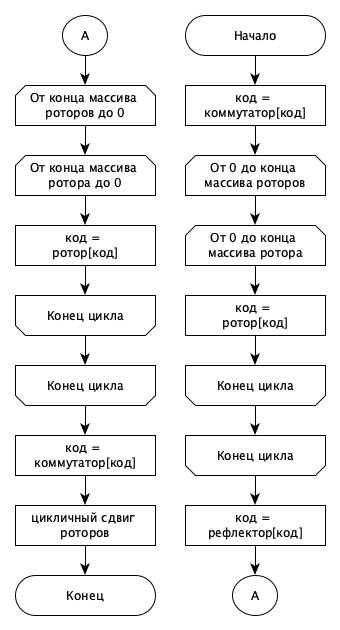
\includegraphics[width=0.6\linewidth]{img/graphs/enigma-algo.png}
	\caption{Схема работы шифровальной машина Энигма}
	\label{fig:alg}
\end{figure}

\section{Модификация алгоритма}

Классический алгоритм предусматривает шифрование произвольного текста, состоящего из печатных символов.
Однако для обеспечения возможности шифровать произвольные бинарные файлы необходимо модифицировать классический алгоритм одним из двух способов.

\begin{enumerate}
    \item Дополнить алгоритм преобразованием бинарных данных в текстовый формат (например, с помощью алгоритма base64).
    
    Однако в этом случае, алгоритмы шифрования и дешифровки будут разными, так как данное преобразование необходимо производить перед шифрованием и только для бинарных данных, и после дешифровки.

    \item Расширить алфавит используемый в алгоритме до 256 символов.
    
    В этом случае идентичность процессов шифрования и дешифровки сохранится, а текстовые и бинарные данные будут обрабатываться одинаково.
\end{enumerate}

В данной лабораторной работе применяется второй из описанных способов, как более простой и понятный в реализации.

\clearpage
